\documentclass[../main.tex]{subfiles}
\begin{document}
\section{Introduction}
\label{sec:intro}
In data visualization it is assumed the graphical representation of data match the properties of the data, and in this work we propose that the mathematical notion of equivariance formalizes this expectation. We meld the infoviz communities interest in heterogenous often discrete datasets with the scientific visualization communities emphasis on continuous and sometimes topologically complex datasets. To demonstrate the practical value of our model, we propose a model driven re-architecture of the artist layer of the Python visualization library Matplotlib. In addition to providing a way to ensure the library preserves structure, we propose a functional approach to  improve modularity, maintainability, and point to ways in which the library could better support concurrency and interactivity.

\section{Background}
\begin{figure}[H]
    \begin{subfigure}{.24\textwidth}
        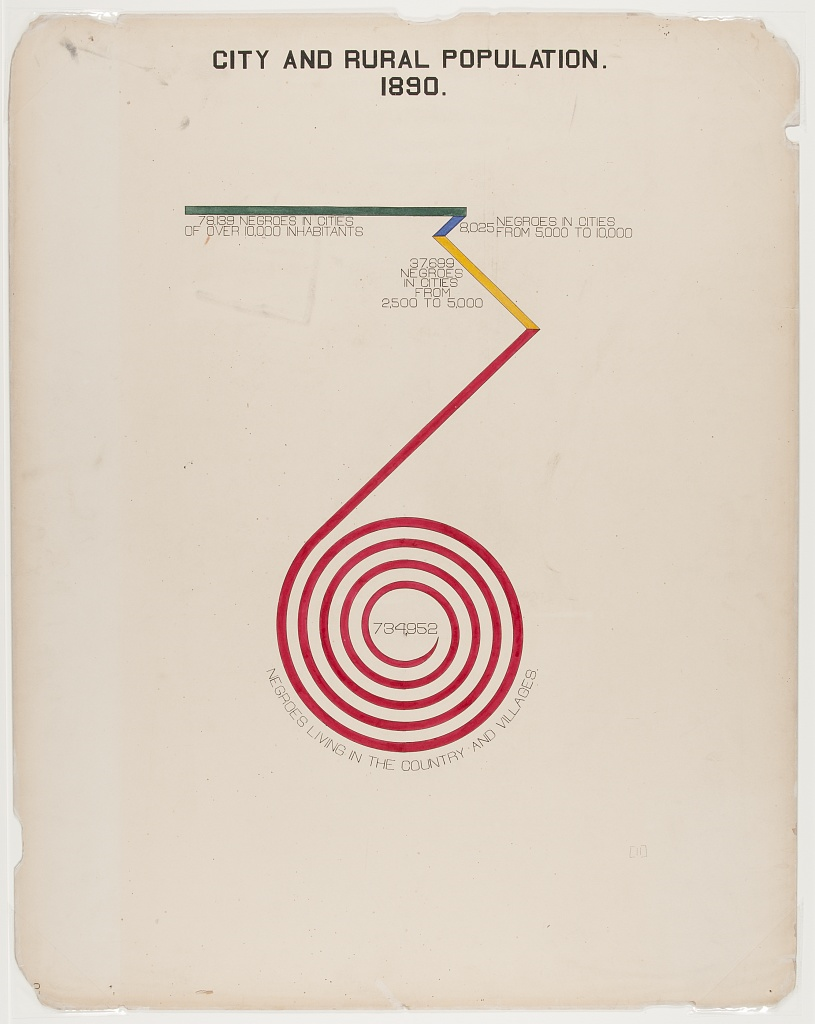
\includegraphics[width=1\textwidth]{figures/intro/du_bois_spinny.png}
        \caption{}
        \label{fig:intro_dpa}
    \end{subfigure}
    \begin{subfigure}{.24\textwidth}
        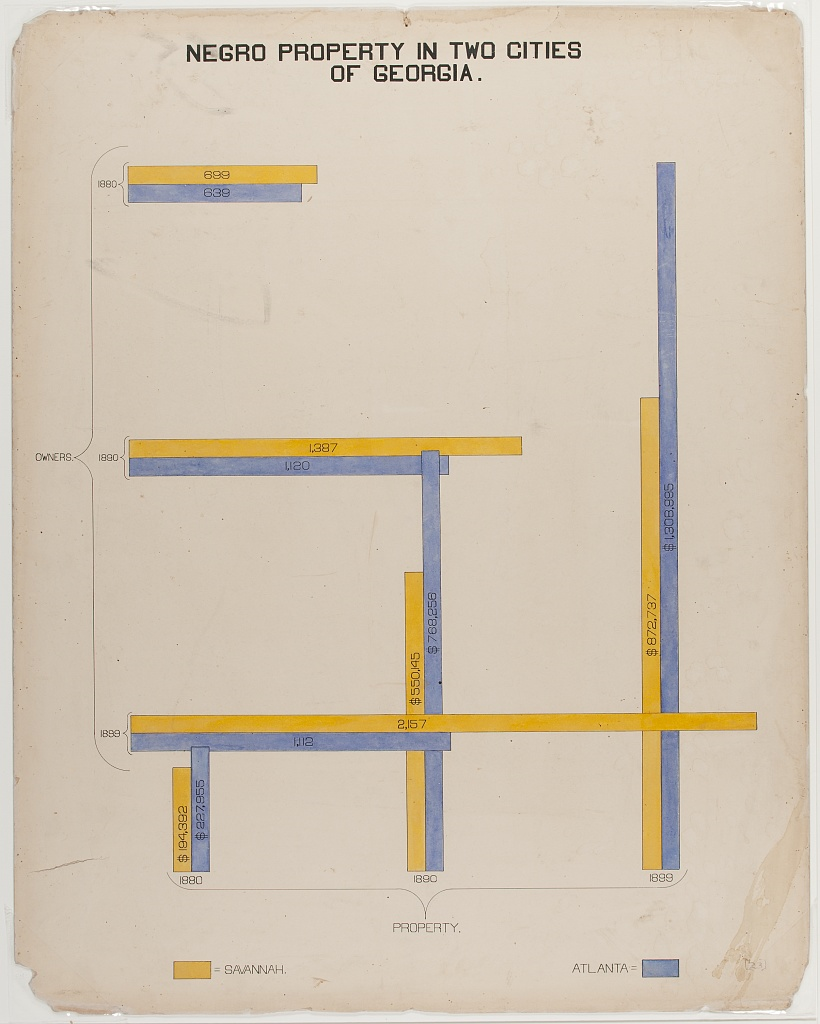
\includegraphics[width=1\textwidth]{figures/intro/du_bois_bar.png}
        \caption{}
        \label{fig:intro_dpb}
    \end{subfigure}
    \begin{subfigure}{.24\textwidth}
        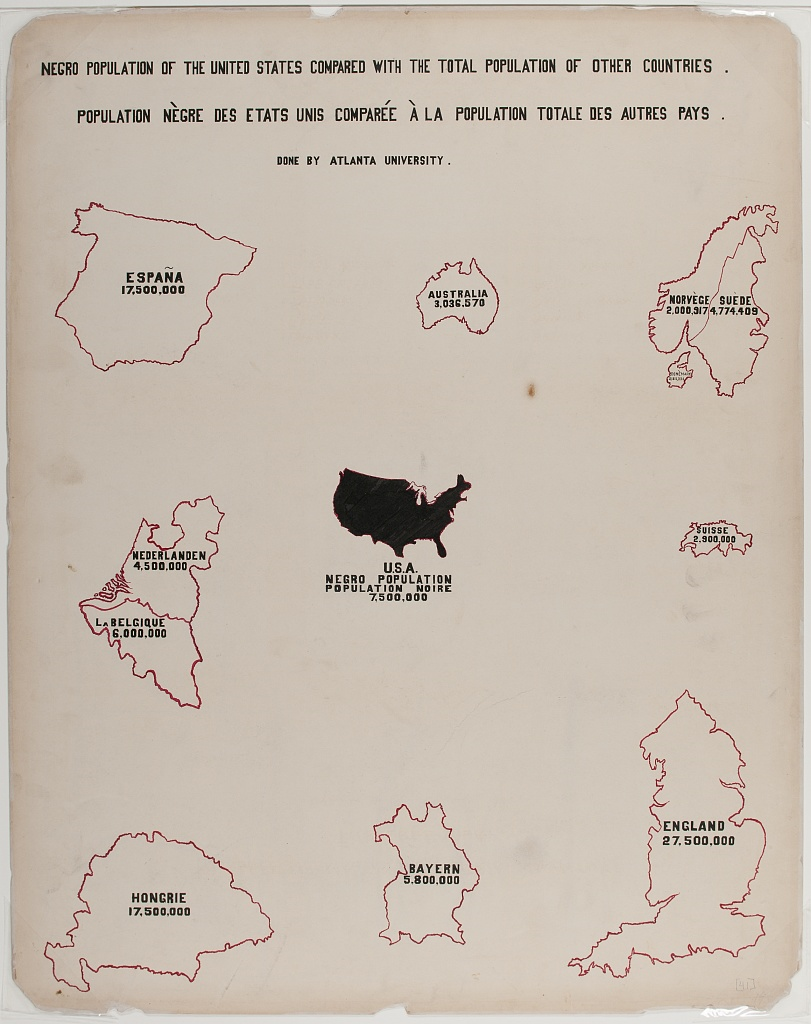
\includegraphics[width=1\textwidth]{figures/intro/du_bois_country.png}
        \caption{}
        \label{fig:intro_dbc}
    \end{subfigure}
    \begin{subfigure}{.24\textwidth}
        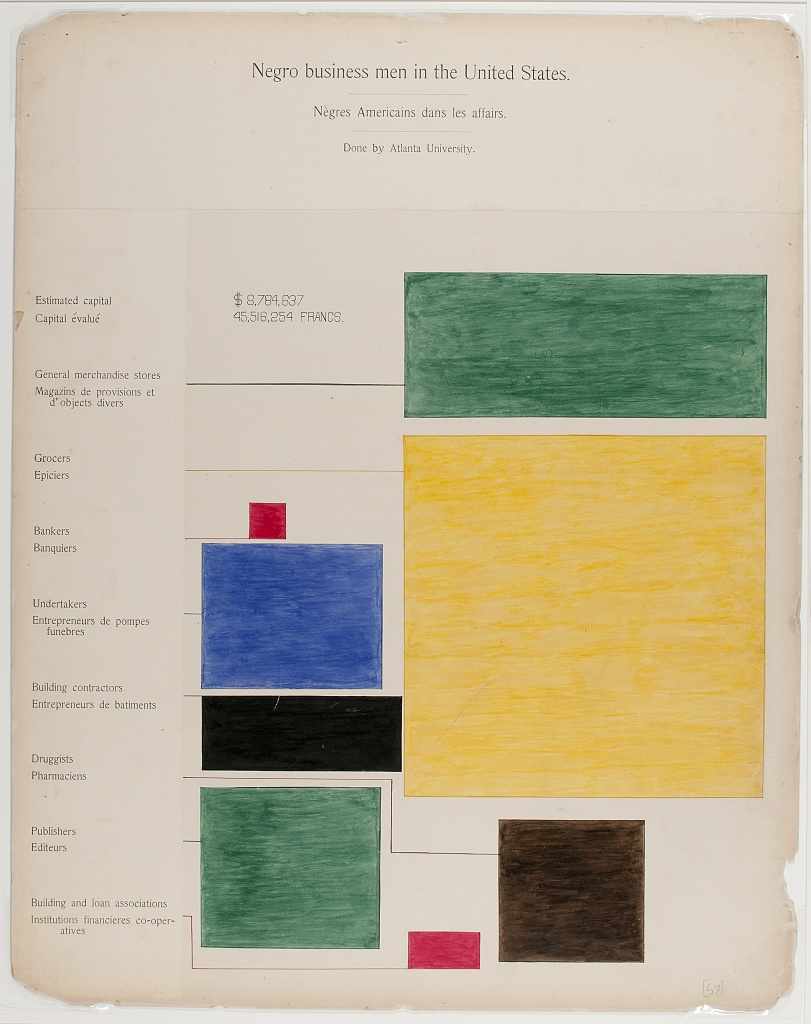
\includegraphics[width=1\textwidth]{figures/intro/du_bois_heat.png}
        \caption{}
        \label{fig:intro_dbd}
    \end{subfigure}
    \caption{Du Bois' data portraits\cite{duboiscenterattheuniversityofmassachusettsBoisDataPortraits2018} of post reconstruction Black American life exemplify that the fundemental characteristics of data visualization is that the visual elements vary in proportion to the source data. In figure~\ref{fig:intro_dpa}, the length of each segment maps to population; in figure~\ref{fig:intro_dpb}, the bar charts are intersected to show the number of property owners and how much they own in a given year; in figure~\ref{fig:intro_dbc} the countries are scaled to population size; and figure~\ref{fig:intro_dbd} is a treemap where the area of the rectangle is representative of the number of businesses in each field. The images here are from the Prints and Photographs collection of the Library of Congress \cite{duboisGeorgiaNegroCity1900,duboisGeorgiaNegroNegro1900, duboisSeriesStatisticalCharts, duboisSeriesStatisticalChartsa}}
    \label{fig:intro_dubois}
\end{figure}

This work aims to develop a model of visualization such that a tool built using this model could support visualizations as varied as those of Du Bois in figure~\ref{fig:intro_dubois}; to do so, we first discuss the criteria by which a visualization is evaluated. Byrne et al. propose that visualizations have graphic representations that are mappings from data to visuals and figurative representations that have meaning due to their similarity in shape to external concepts \cite{byrneAcquiredCodesMeaning2016}. In figure~\ref{fig:intro_dbc}, Du Bois combines a graphical representation where glyph size varies by population with a figurative representation of those glyphs as the countries the data is from, which means that the semantic and numerical properties of the data are preserved in the graph. Tufte specifies that visual representations must be in proportion to the quantitative data being represented for a chart to be faithful and that there should be no extra information in the graphic or figurative elements of the graph, but otherwise his notion of graphic integrity is heavily context dependent\cite{tufteVisualDisplayQuantitative2001}. As is Norman's Naturalness Principal, which states that visualizations are more understandable  when the properties of the representation match the properties of the information being represented\cite{norman_things_smart}. Bertin takes it as a given that data properties match visual properties, so much so that Munzner argues it is inherently built into his classification system \cite{munznerVisualizationAnalysisDesign2014} which is displayed in figure~\ref{fig:intro_retinal_variables}.

\begin{figure}[H]
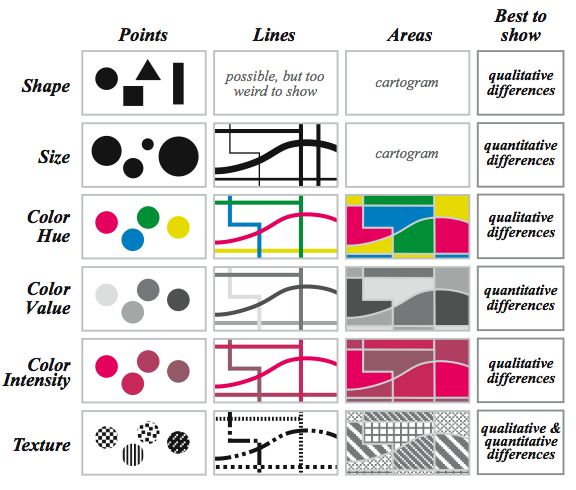
\includegraphics[width=1\textwidth]{figures/intro/retinal_variables.png}
\caption{Retinal variables are a codification of how position, size, shape, color and texture are used to illustrate variations in the components of a visualization. The best to show column describes which types of information can be expressed in the corresponding visual encoding. This tabular form of Bertin's retinal variables is from Understanding Graphics \cite{malamedInformationDisplayTips2010} who reproduced it from \textit{Making Maps: A Visual Guide to Map Design for GIS} 
\cite{krygierMakingMapsVisual2005}}
\label{fig:intro_retinal_variables}
\end{figure}

As described by Mackinlay, a visualization tool produces a graphical design and an image rendered based on that design. He defines the graphical design as the set encoding relations from data to visual representation\cite{mackinlayAutomatingDesignGraphical1986}, and the design rendered in an idealized abstract space is what throughout this paper we will refer to as a graphic. Mackinlay  proposes that a visualization tool's expressiveness is a measure of how much of the structure of the data the tool encodes, while the tools effectiveness describes how much design choices are made in deference to perceptual saliency \cite{clevelandResearchStatisticalGraphics1987,clevelandGraphicalPerceptionTheory1984,chambersGraphicalMethodsData1983a, munznerVisualizationAnalysisDesign2014}. Mackinlay's definition of expressiveness is formalized at the visual encoding level, which as shown in figure~\ref{fig:intro_retinal_variables} refers to the components of a graphic such as the color or position of a glyph. Bertin first classified these graphic components as retinal variables and discussed which types of data they can express \cite{bertinIIPropertiesGraphic2011} and how they are composited on point, line, and area graphical marks, as shown in figure~\ref{fig:intro_retinal_variables} correspond. Marks can be generalized to glyphs, which are graphical objects that convey one or more attributes of the data entity mapped to it\cite{ware2019information}. Mackinlay's expressiveness criteria is well defined for the visual variables, such that he suggests the viability of a strict encoding relation that is a homomorphic mapping which preserves some binary operator from one domain to another \cite{mackinlayAUTOMATICDESIGNGRAPHICAL1987}. We expand on this suggestion by proposing that monoid action equivariance is a strict condition of building valid encoders. Mackinlay does not provide a generalized criteria for plot types, instead embedding the requirements within the definition of the charts. 


\subsection{Data}
\label{sec:intro_data}
Tory and Möller propose that assumptions about the structure of data are built into the visual algorithms that display that information \cite{toryRethinkingVisualizationHighLevel2004}. Specifically they note that discrete and continuous data and their attributes form a discipline independent design space \cite{pousmanCasualInformation2007}. 

\begin{figure}[H]
    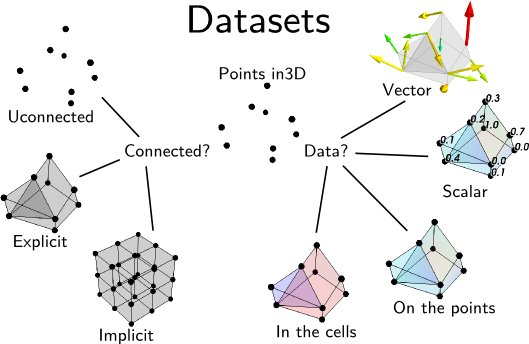
\includegraphics[width=1\textwidth]{figures/intro/dataset_diagram.png}
    \caption{One way to describe data is by the connectivity of the points in the dataset. A database for example is often discrete unconnected points, while an image is an implicitely connected 2D grid. This image is from the Data Representation chapter of the MayaVi 4.7.2 documentation.\cite{DataRepresentationMayavi}}
    \label{fig:intro_data_format}
\end{figure}


As shown in figure~\ref{fig:intro_data_format}, there are many types of continuity in data. A database typically consists of unconnected records, while an image is an implicit 2D grid and a network is some sort of explicitly connected graph. In this work we will refer to the points of the dataset as \textit{records} to indicate that a point can be a vector. Each \textit{component} of the record is a single object, such as a temperature, a color, or an image. The way in which these records are connected is the \textit{connectivity}, \textit{continuity}, or more generally \textit{topology}. 
\begin{figure}[H]
    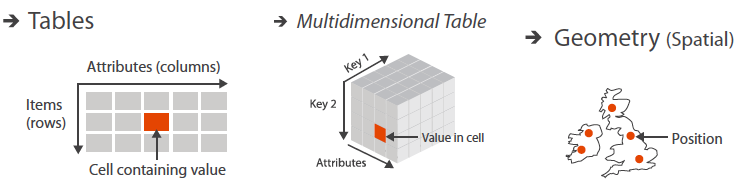
\includegraphics[width=\textwidth]{figures/intro/munzner_datatypes}
   \caption{Keys are unique lookup values used to find individual observations in the dataset. Keys are positional references, and can be coordinates on a map or unique values such as a primary key in a database or a (time, latitude, longitude) index in a data cube. Image modified from a diagram from Munzner's \textit{Visualization Analysis and Design} \cite{munznerVisualizationAnalysisDesign2014}}
   \label{fig:intro_munzner_datatypes}
   \end{figure}

Often this topology has metadata associated with it, as shown in figure~\ref{fig:intro_munzner_datatypes}. Munzner denotes this metadata as \textit{keys} that can be used to locate the record, and further to locate the specific \textit{value} \cite{munznerChDataAbstraction}. In figure~\ref{fig:intro_munzner_datatypes} tables have keys identifying the row and column and sometimes also the depth, while maps have a location key. We propose that information rich keys such as location are additional components of the record, and that instead there are coordinate free structural keys that identify the location of the record within a dataset of any continuity. 

In this work, we extend Butler's topology driven representation of visualization data \cite{butlerVisualizationModelBased1989,butlerVectorBundleClassesForm1992}. Butler proposes that fiber bundles are a good model for visualization data because it allows for encoding the connectivity seperately from the records and supports discrete and ND continuous datasets. Since Butler's model lacks a robust way of describing the components of the record, we fold in Spivak's Simplacial formulation of databases \cite{spivakDatabasesAreCategories2010,spivakSIMPLICIALDATABASES} so that we can encode a schema like discription of the data in the fiber bundle. We then propose criteria on expressivity that take into account both the components and the continuity of the data. 

\subsection{Tools}
\label{sec:intro_data_tools}
 
A motivator for this work is that currently Matplotlib carries implicit assumptions about data continuity in how each function interfaces with the input data. This work proposes a unified internal representation that encodes connectivity in a common interface. Matplotlib aims to natively support data of varying connectivities, so tools primarily concerned with visualizing relational data of the type found in databases are insufficient models. Many of these tools are built on top of Wilkenson's Grammar of Graphics \cite{wilkinsonGrammarGraphics2005} which itself incorporates Mackinlay's  A Presentation Tool (APT) display algebra; GoG derivative include ggplot\cite{wickhamGgplot2ElegantGraphics2016a}, protovis\cite{bostockProtoviz2009} and D3 \cite{bostockDataDrivenDocuments2011}, vega\cite{satyanarayanDeclarativeInteractionDesign2014} and altair\cite{vanderplasAltairInteractiveStatistical2018}. While many of these tools support images, the first class data container is a table like object of discrete records. Tools that primarily support images are also insufficient. For example ImageJ\cite{schneiderNIHImageImageJ2012} and the ImagePlot\cite{studiesCulturevisImageplot2021}macro have some support for visualizing non image components of a complex data set, but mostly in service to the image being visualized. Plugins exist, but must work around the everything is an image data model\cite{WritingPlugins}. There are also visualization tools that do not carry implicit assumptions about structure, for example vtk\cite{hanwellVisualizationToolkitVTK2015,geveci2012vtk} and its derivatives such as MayaVi\cite{ramachandranMayaVi2011}. \note{Not totally positive but I think VTK is deeply coupled to the renderer and that's why we're not using it as a model, but not positive and this is literally what Marc worked on...}


\subsection{contribution}
The contribition of this work is a model we call the topological artist model (TAM) in which data and graphics can be viewed as sections of fiber bundles. This model allows for (1) decomposing the translation of data fields (variables) into visual channels via an equivariant map on the fibers and (2) a topology-preserving map of the base spaces that translates the dataset connectivity into graphical elements. Furthermore, this model supports an algebraic sum operation such that more complex visualizations can be built from simple ones. To demonstrate the practical value of the model, we built a prototype where we represent the topological base spaces using triangulation, make use of programming types for the fiber, and build on Matplotlib's existing infrastructure for the rendering. 
\end{document}